\clearpage
\twocolumn[{%
\rqparent
\subsection{Decision accuracy across sizes}
\label{app:rq02_decision_accuracy}

\noindent\begin{minipage}[t]{0.485\textwidth}
\vspace{0pt}
\paragraph{Research Question.} \emph{Decision accuracy (DA), the framework's ground truth, is the probability that a benchmark orders a pair of models as an evaluation of larger models would (Heineman et al., 2025). Which benchmarks, in which languages, keep the ranking of the ladder's design variants across sizes (\textbf{DA-size}), along training (\textbf{DA-ckpt}), and early \emph{and} small at once (\textbf{DA-goal})?}

\paragraph{Setup.} We measure DA-size, the share of design pairs that a proxy's final checkpoint (90M--1B) orders like the 1.7B reference's. We use the seed-1904 runs of every language setting, ladder and data build. A pair differs on one design axis or several. The tasks are the benchmark tasks above chance at the proxy and at 1.7B with at least three comparable pairs, their bBPB twins (the gold answer's bits per byte on the same items, figure: app\_rq02\_bbpb), and the per-language BPB of the 50 trained languages. A line divides matching by comparable decisions, summed over its tasks. We map DA per benchmark and language (Figures~\ref{fig:app_rq02_da_by_language} and~\ref{fig:app_rq02_da_size_by_language_per_proxy}). We pick, out of sample, the tasks with median DA-size or DA-ckpt $\geq$ 0.66 (Figures~\ref{fig:app_rq02_rq2_crossfit} and~\ref{fig:app_rq02_decision_accuracy_crossfit}). We compare the proxies with the agreement of two seeds of one design (Figure~\ref{fig:app_rq02_seed_uncertainty}).
\end{minipage}\hfill
\begin{minipage}[t]{0.485\textwidth}
\vspace{0pt}
\begin{rqfinding}
\textbf{1. A smaller fully trained model ranks the design variants close to chance.} On benchmark accuracy alone, DA-size is 0.51, 0.53, 0.52, 0.54 and 0.56 from 90M to 1B (mean over 359--553 gated tasks), and no proxy comes near the 0.90 threshold (Table~\ref{tab:app_rq02_definition_sensitivity}). (Figure~\ref{fig:app_rq02_decision_accuracy}.)
\\
\\
\textbf{2. The pooled line in the figure adds the bBPB twins at every size and is flat.} It reads 0.59, 0.57, 0.58, 0.58, 0.58 (90 \% jackknife $\pm$ 0.02--0.03) over 1175--1369 tasks, all 816 twins among them at every size.
\\
\\
\textbf{3. Bits per byte ranks like the reference and accuracy does not.} Per-language BPB reads 0.95, 0.95, 0.91, 0.73, 0.92 from 90M to 1B (mean over 50 per-language tasks) and \texttt{bpb\_macro} 0.94--0.97 (Figure~\ref{fig:app_rq02_bbpb_acc_gate}).
\end{rqfinding}
\end{minipage}

\vspace{\baselineskip}
\noindent\begin{minipage}{\textwidth}
\centering
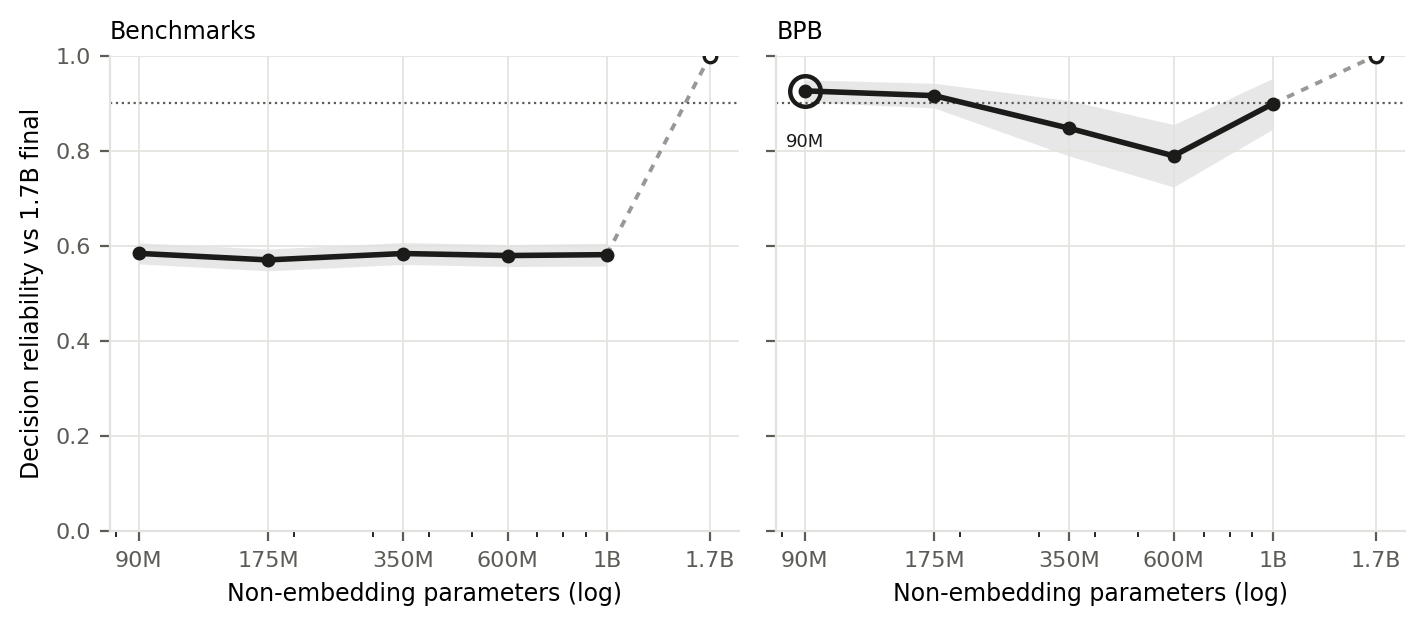
\includegraphics[width=\textwidth,height=0.36\textheight,keepaspectratio]{figures/app_rq02_decision_accuracy.png}
% source: src/signal-and-noise/analysis/rq02_decision_accuracy/pretraining/predictivity/scale_convergence_da_size_multi_axes_paper.png
\captionof{figure}{\textbf{A smaller fully trained model ranks the design variants close to chance.} DA-size of the final checkpoint of each proxy size against the final checkpoint of the 1.7B reference, on multi-axis design pairs, pooled over decisions (matching over comparable pairs, summed over tasks). Left: the benchmark tasks above chance and their bBPB twins. Right: the per-language bits per byte. The band is the 90\% leave-one-variant-out jackknife interval, the dotted line marks 0.9 and the circle marks the smallest proxy above it. The dashed segment joins the 1B proxy to the reference itself.}
\label{fig:app_rq02_decision_accuracy}
\end{minipage}
}]

\begin{figure*}[p]
\centering
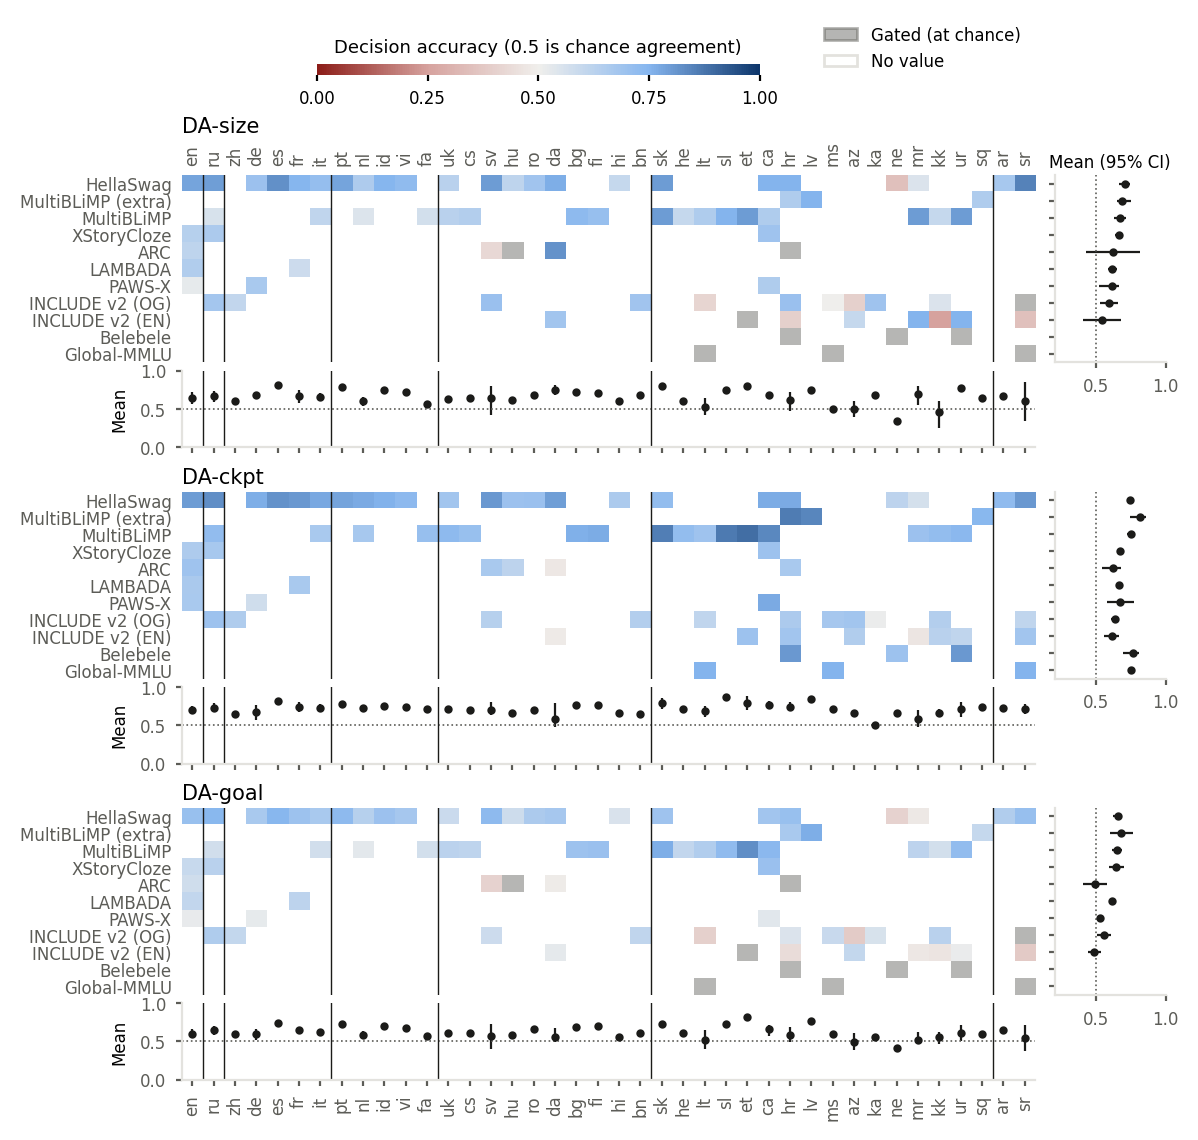
\includegraphics[width=\textwidth,height=0.8\textheight,keepaspectratio]{figures/app_rq02_da_by_language.png}
% source: src/signal-and-noise/analysis/rq02_decision_accuracy/pretraining/predictivity/rq2_da_all_by_benchmark_and_language_above_66_either_mono_axis.png
\caption{\textbf{On the tasks that rank reliably, averaged over the proxies 90M--1B, DA-size is above 0.5 (95\% interval) on 7 of 9 benchmarks and 32 of 40 languages.} DA-goal clears 0.5 on 7 of 9 benchmarks and 31 of 40 languages, DA-ckpt on 11 of 11 and 38 of 40. The mean cell is 0.65 for DA-size, 0.71 for DA-ckpt and 0.61 for DA-goal. Top: DA-size of each proxy's final checkpoint against the 1.7B final. Middle: DA-ckpt of the nine earlier tenths of each run against its own final, over the proxies and the 1.7B run, where DA-ckpt is defined too. Bottom: DA-goal of the ten tenths of each proxy against the 1.7B final. DA-size and DA-goal stop at 1B because 1.7B is their reference. Each task is first averaged over these readings. Side panels: row and column means with 95\% bootstrap intervals over the cells. A cell is the mean over a benchmark's original accuracy tasks (no RF, LLM-RF or bBPB twin) in a trained language, on the mono-axis pairs of Figure~\ref{fig:rq2}. As in that figure, only the tasks whose median DA-size or median DA-ckpt is at least 0.66 are kept. This filter selects on DA, so the maps are conditional on it. Grey cells are gated, white cells have no value, and the scale is centred at 0.5 (chance agreement). Languages follow resource rank, with lines where the lists of $K$ = 1, 2, 8, 15, 30 and 50 languages end. Not drawn are 6 single-language benchmarks.}
\label{fig:app_rq02_da_by_language}
\end{figure*}

\begin{figure*}[p]
\centering
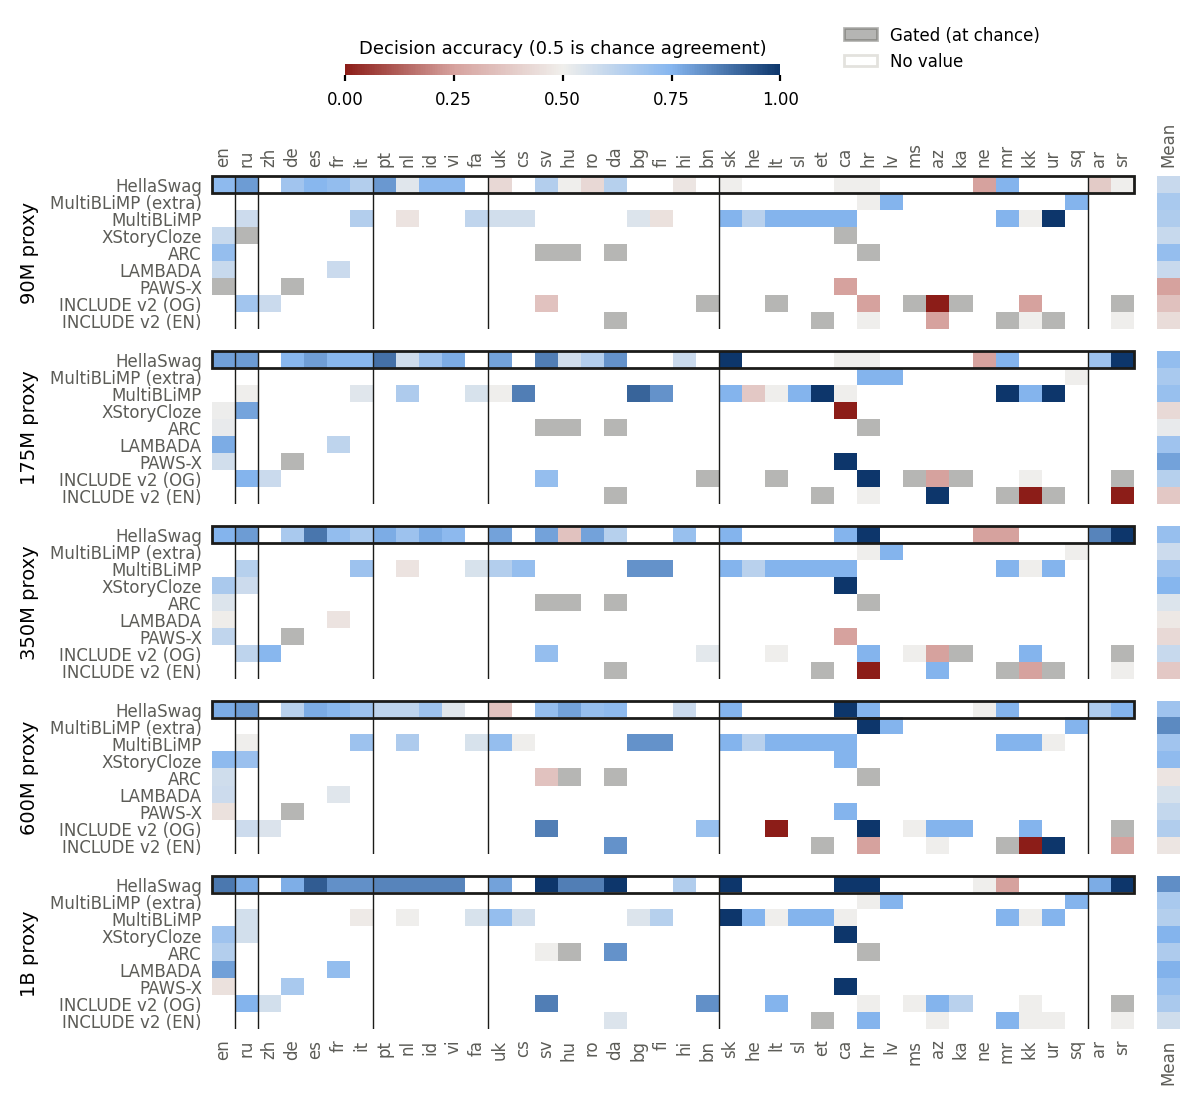
\includegraphics[width=\textwidth,height=0.8\textheight,keepaspectratio]{figures/app_rq02_da_size_by_language_per_proxy.png}
% source: src/signal-and-noise/analysis/rq02_decision_accuracy/pretraining/predictivity/rq2_da_size_by_benchmark_and_language_per_proxy_above_66_either_mono_axis.png
\caption{\textbf{On the tasks that rank reliably, a larger proxy decides more like the 1.7B reference: 60\% of the cells with a value have DA-size above 0.5 at 90M and 76\% at 1B, and HellaSwag (outlined) is above 0.5 at every proxy in 12 of its 23 languages.} The mean goes from 0.57 to 0.71. Without the filter it goes only from 0.52 to 0.56. DA-size of each proxy's final checkpoint against the 1.7B final, one map per proxy, with the row means in the last map. Only benchmarks with a DA-size at some proxy are drawn. A cell is the mean over a benchmark's original accuracy tasks (no RF, LLM-RF or bBPB twin) in a trained language, on the mono-axis pairs of Figure~\ref{fig:rq2}. As in that figure, only the tasks whose median DA-size or median DA-ckpt is at least 0.66 are kept. This filter selects on DA, so the maps are conditional on it. Grey cells are gated, white cells have no value, and the scale is centred at 0.5 (chance agreement). Languages follow resource rank, with lines where the lists of $K$ = 1, 2, 8, 15, 30 and 50 languages end. Not drawn are 6 single-language benchmarks, and Belebele, Global-MMLU, which have no value.}
\label{fig:app_rq02_da_size_by_language_per_proxy}
\end{figure*}

\begin{figure*}[p]
\centering
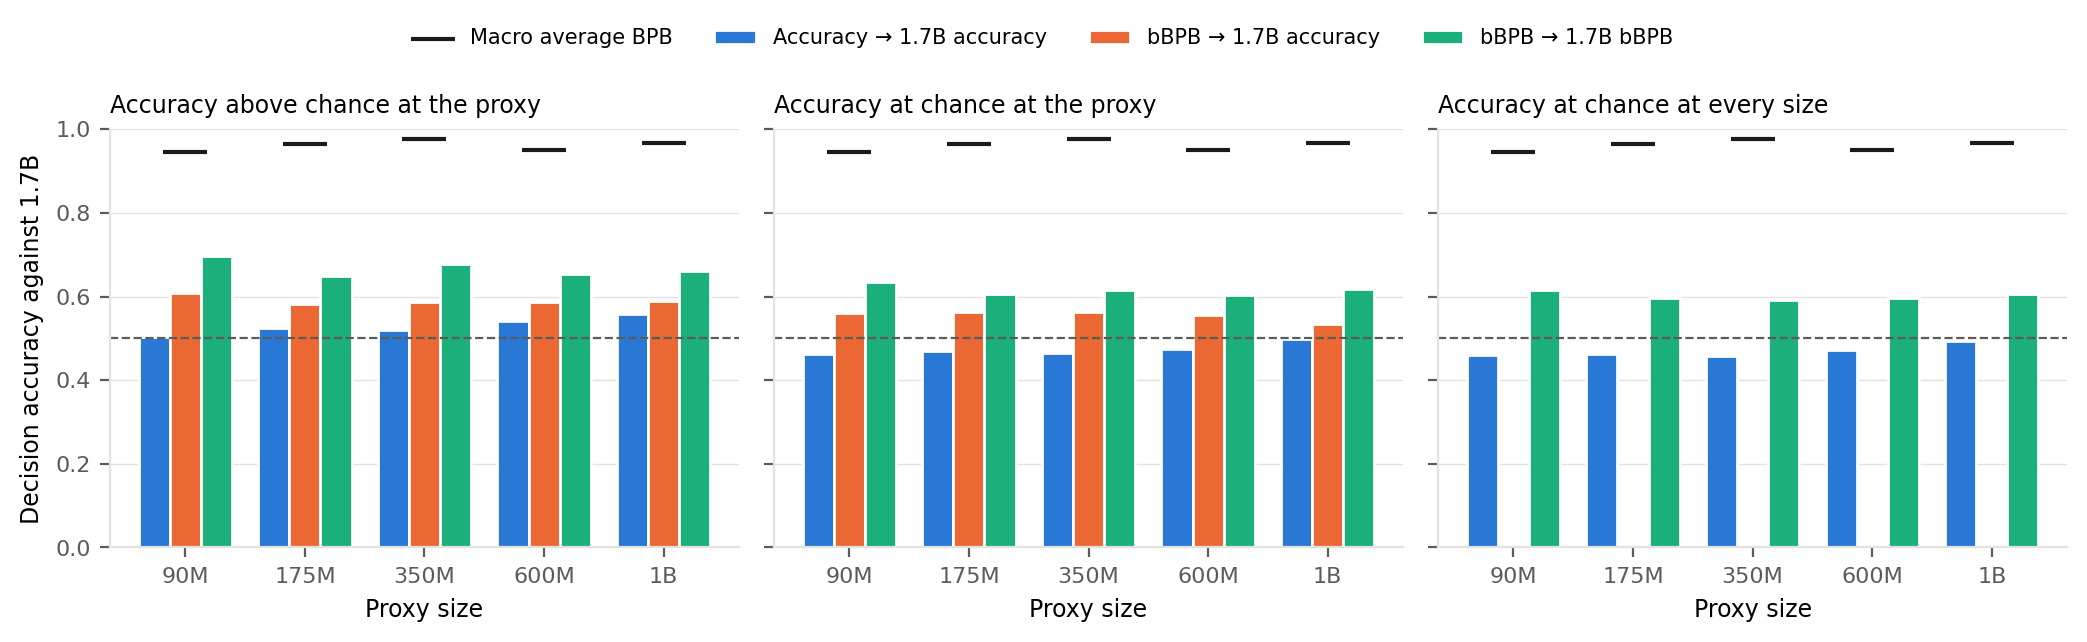
\includegraphics[width=\textwidth,height=0.8\textheight,keepaspectratio]{figures/app_rq02_bbpb_acc_gate.png}
% source: src/signal-and-noise/analysis/rq02_decision_accuracy/pretraining/predictivity/bench_bpb_da_size_by_acc_gate_multi_axes_paper.png
\caption{\textbf{Where accuracy is at chance at the proxy, bBPB still ranks the design variants like the 1.7B bBPB at 0.60--0.63, above accuracy on the same tasks (0.46--0.50) but far below the bits per byte of the training languages (0.95--0.98).} DA-size of the final checkpoint of each proxy against the 1.7B final checkpoint, on multi-axis design pairs, over the benchmark tasks split by their accuracy: above chance at the proxy (left), at chance at the proxy (middle) and, a subset of the middle, at chance at every size (right). The pairs are the 406 of the 528 multi-axis pairs whose two families the per-item store holds. Blue: accuracy against the 1.7B accuracy, without the above-chance filter. Orange: the bBPB of the proxy against the 1.7B accuracy, defined where the 1.7B accuracy is above chance (0.53--0.56 in the middle panel). Green: bBPB against the 1.7B bBPB, which has no chance level. The middle panel holds 532 tasks at 90M and 360 at 1B. The black tick is the DA-size of the macro average of the per-language bits per byte on the same pairs, and the dashed line marks 0.5.}
\label{fig:app_rq02_bbpb_acc_gate}
\end{figure*}

\begin{figure*}[p]
\centering
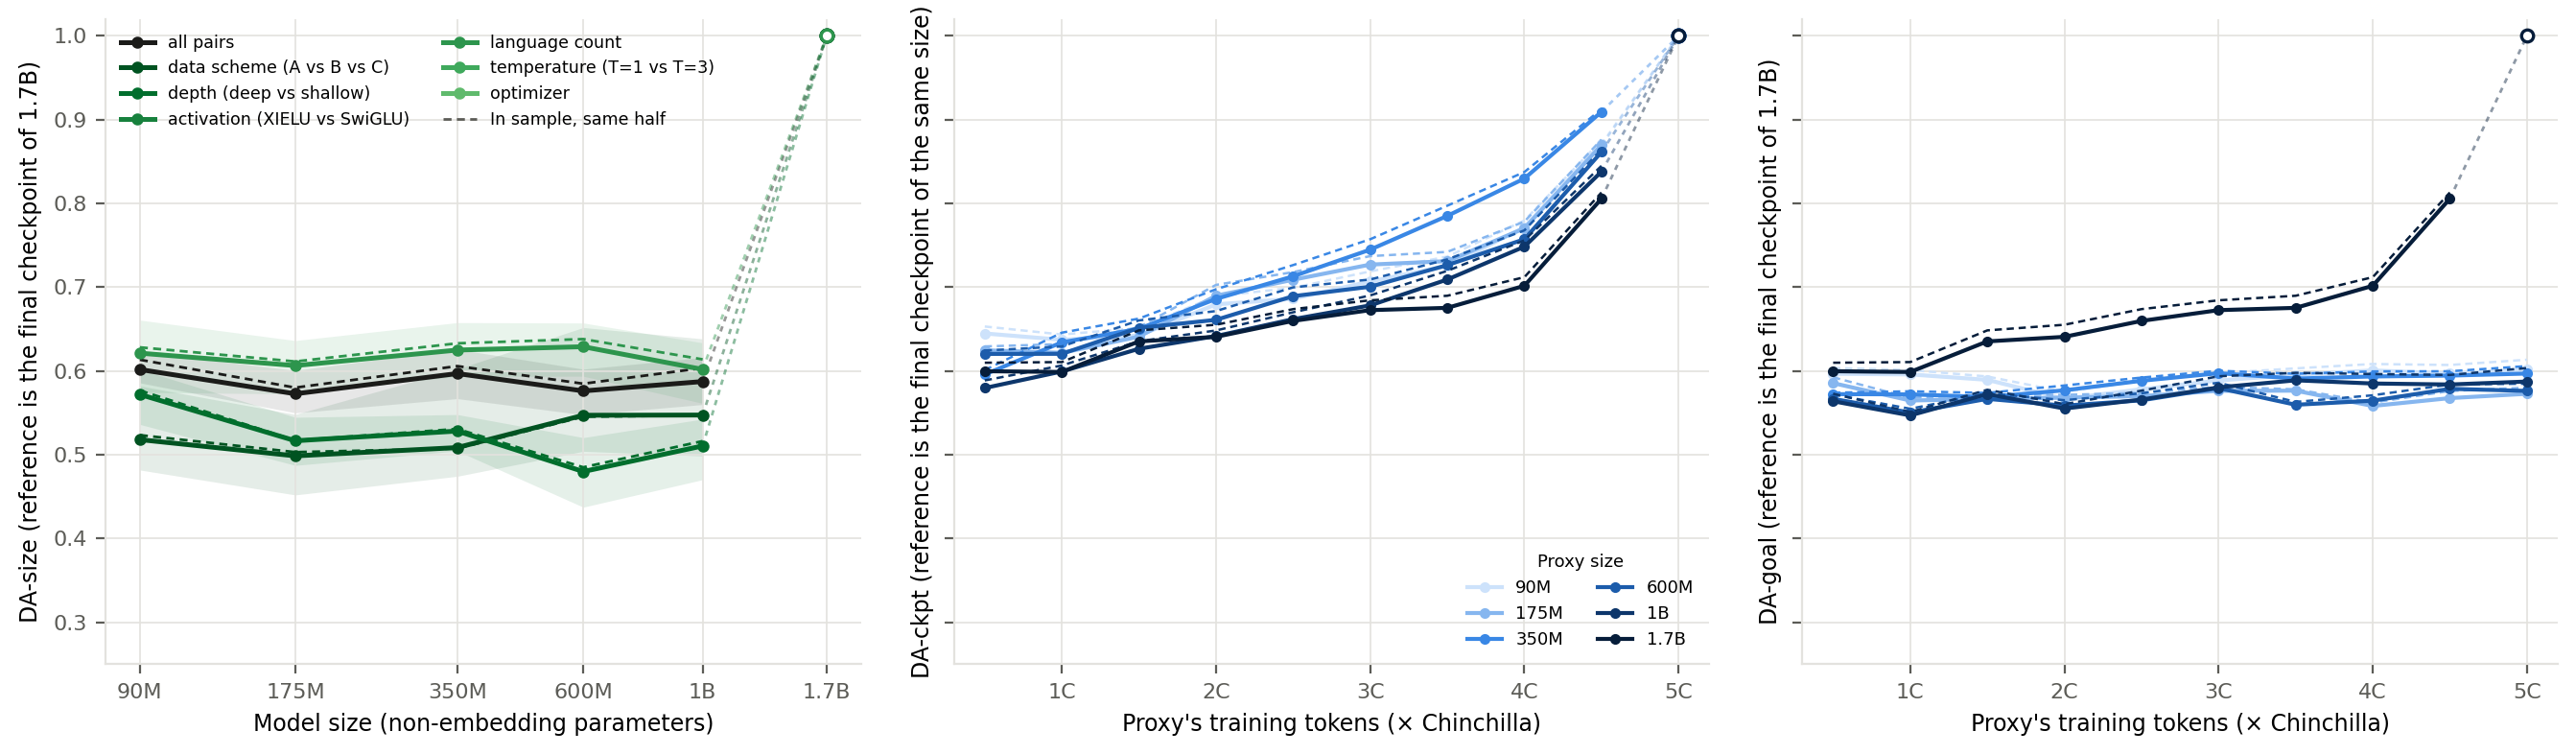
\includegraphics[width=\textwidth,height=0.8\textheight,keepaspectratio]{figures/app_rq02_rq2_crossfit.png}
% source: src/signal-and-noise/analysis/rq02_decision_accuracy/pretraining/predictivity/rq2_da_all_above_66_either_crossfit_transformation_mono_axis.png
\caption{\textbf{Choosing the reliable tasks out of sample moves DA-size over all single-axis pairs by at most 0.02 (at 1B).} Figure~\ref{fig:rq2} redrawn with the reliable tasks chosen out of sample. We decide which tasks are reliable (DA above 0.66 on the size or the checkpoint axis) on one half of the design pairs and read the panels on the other half. We repeat this over 20 random splits, stratified by the axes a pair moves, and in both directions (solid lines, with the 5--95\% range over splits). The dashed lines choose and read the tasks on the same half, so the gap between solid and dashed lines is the selection effect alone. Lines with too few pairs per half are not drawn.}
\label{fig:app_rq02_rq2_crossfit}
\end{figure*}

\begin{figure*}[p]
\centering
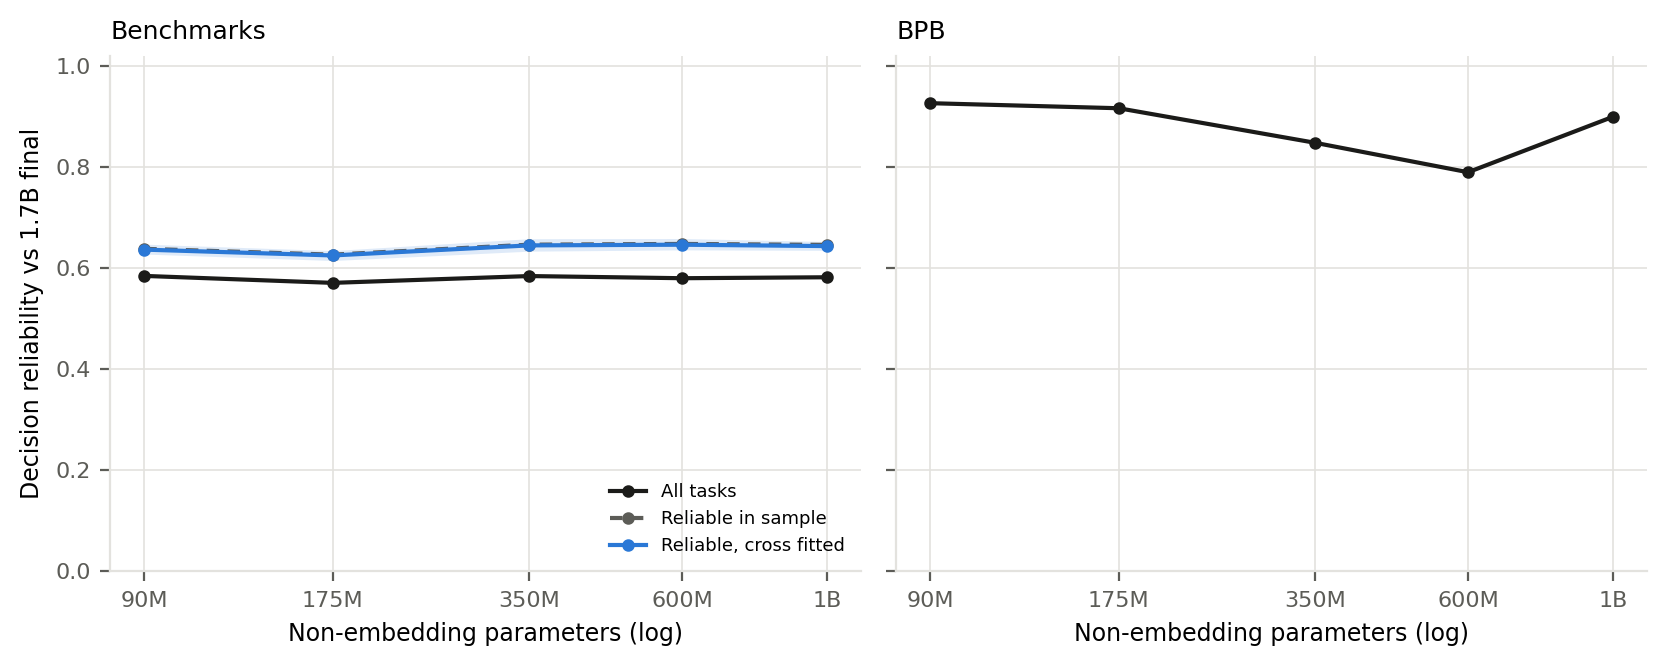
\includegraphics[width=\textwidth,height=0.8\textheight,keepaspectratio]{figures/app_rq02_decision_accuracy_crossfit.png}
% source: src/signal-and-noise/analysis/rq02_decision_accuracy/pretraining/predictivity/scale_convergence_da_size_above_66_either_crossfit_multi_axes_paper.png
\caption{\textbf{On the multi-axis pairs, the reliable benchmark tasks chosen out of sample and in sample give DA-size within 0.00 of each other.} Figure~\ref{fig:app_rq02_decision_accuracy} redrawn with the reliable benchmark tasks chosen out of sample (solid) or in sample on the same half of the pairs (dashed), over the splits of Figure~\ref{fig:app_rq02_rq2_crossfit}.}
\label{fig:app_rq02_decision_accuracy_crossfit}
\end{figure*}

\begin{table*}[p]
\centering
\small
\begin{adjustbox}{max width=\textwidth}
\begin{tabular}{lrrrrrr}
\toprule
Definition & Pairs kept & 90M & 175M & 350M & 600M & 1B \\
\midrule
\multicolumn{7}{l}{\textit{Benchmark accuracy}} \\
Current rule (a pair tied on one side misses) & 100\% & 0.51 & 0.53 & 0.53 & 0.54 & 0.56 \\
A tied pair counts one half & 100\% & 0.54 & 0.56 & 0.56 & 0.57 & 0.59 \\
Pairs the reference ties dropped & 96\% & 0.52 & 0.54 & 0.53 & 0.55 & 0.57 \\
Reference gap $>$ 1 reference checkpoint SD & 72\% & 0.54 & 0.56 & 0.55 & 0.57 & 0.59 \\
Reference gap $>$ 2 reference checkpoint SD & 47\% & 0.55 & 0.56 & 0.57 & 0.61 & 0.62 \\
Reference gap $>$ 1 seed SD of a difference & 51\% & 0.55 & 0.56 & 0.57 & 0.60 & 0.62 \\
Reference gap $>$ 2 seed SD of a difference & 23\% & 0.59 & 0.60 & 0.62 & 0.65 & 0.67 \\
\midrule
\multicolumn{7}{l}{\textit{Benchmark accuracy and bBPB twins}} \\
Current rule (a pair tied on one side misses) & 100\% & 0.62 & 0.59 & 0.61 & 0.60 & 0.61 \\
A tied pair counts one half & 100\% & 0.62 & 0.60 & 0.62 & 0.61 & 0.62 \\
Pairs the reference ties dropped & 99\% & 0.62 & 0.60 & 0.61 & 0.60 & 0.62 \\
Reference gap $>$ 1 reference checkpoint SD & 73\% & 0.65 & 0.62 & 0.64 & 0.63 & 0.64 \\
Reference gap $>$ 2 reference checkpoint SD & 50\% & 0.68 & 0.65 & 0.67 & 0.66 & 0.67 \\
Reference gap $>$ 1 seed SD of a difference & 47\% & 0.68 & 0.64 & 0.67 & 0.66 & 0.68 \\
Reference gap $>$ 2 seed SD of a difference & 21\% & 0.73 & 0.70 & 0.73 & 0.71 & 0.73 \\
\midrule
\multicolumn{7}{l}{\textit{Per-language BPB}} \\
Current rule (a pair tied on one side misses) & 100\% & 0.94 & 0.94 & 0.89 & 0.74 & 0.92 \\
A tied pair counts one half & 100\% & 0.94 & 0.94 & 0.89 & 0.74 & 0.92 \\
Pairs the reference ties dropped & 100\% & 0.94 & 0.94 & 0.89 & 0.74 & 0.92 \\
Reference gap $>$ 1 reference checkpoint SD & 79\% & 0.98 & 0.98 & 0.94 & 0.79 & 0.96 \\
Reference gap $>$ 2 reference checkpoint SD & 58\% & 1.00 & 1.00 & 0.98 & 0.93 & 1.00 \\
Reference gap $>$ 1 seed SD of a difference & 70\% & 0.99 & 0.99 & 0.95 & 0.86 & 0.97 \\
Reference gap $>$ 2 seed SD of a difference & 48\% & 1.00 & 1.00 & 0.98 & 0.99 & 1.00 \\
\bottomrule
\end{tabular}

\end{adjustbox}
% source: src/signal-and-noise/analysis/rq02_decision_accuracy/pretraining/predictivity/da_size_definition_sensitivity_multi_axes.tex
\caption{\textbf{No definition of decision accuracy lifts benchmark accuracy far above chance.} DA-size of the final checkpoint of each proxy against the 1.7B final checkpoint, on multi-axis pairs, under the definition of Eq.~\ref{eq:decision-accuracy} and its variants: a tied pair (on one side or both) counts one half, the pairs the reference ties are dropped, or only the pairs whose 1.7B difference exceeds one or two checkpoint standard deviations of the reference (over the last 20\% of its run, detrended) or one or two seed standard deviations of a difference are kept. A value is the mean over the tasks above chance at the proxy and at 1.7B, for benchmark accuracy, for accuracy and the bBPB twins together, and for the per-language bits per byte, which never tie. Pairs kept is the share of the comparable pairs a variant keeps, pooled over the proxy sizes. The task set moves across rows, since a cell needs three kept pairs: on accuracy it holds 359--553 tasks per proxy under Eq.~\ref{eq:decision-accuracy} and 243--387 under the strictest filter. A value is a mean over tasks, so it can differ from the pooled lines of Figures~\ref{fig:app_rq02_decision_accuracy} and \ref{fig:app_rq02_decisive_pairs}, which weigh a task by its pairs.}
\label{tab:app_rq02_definition_sensitivity}
\end{table*}

\begin{figure*}[p]
\centering
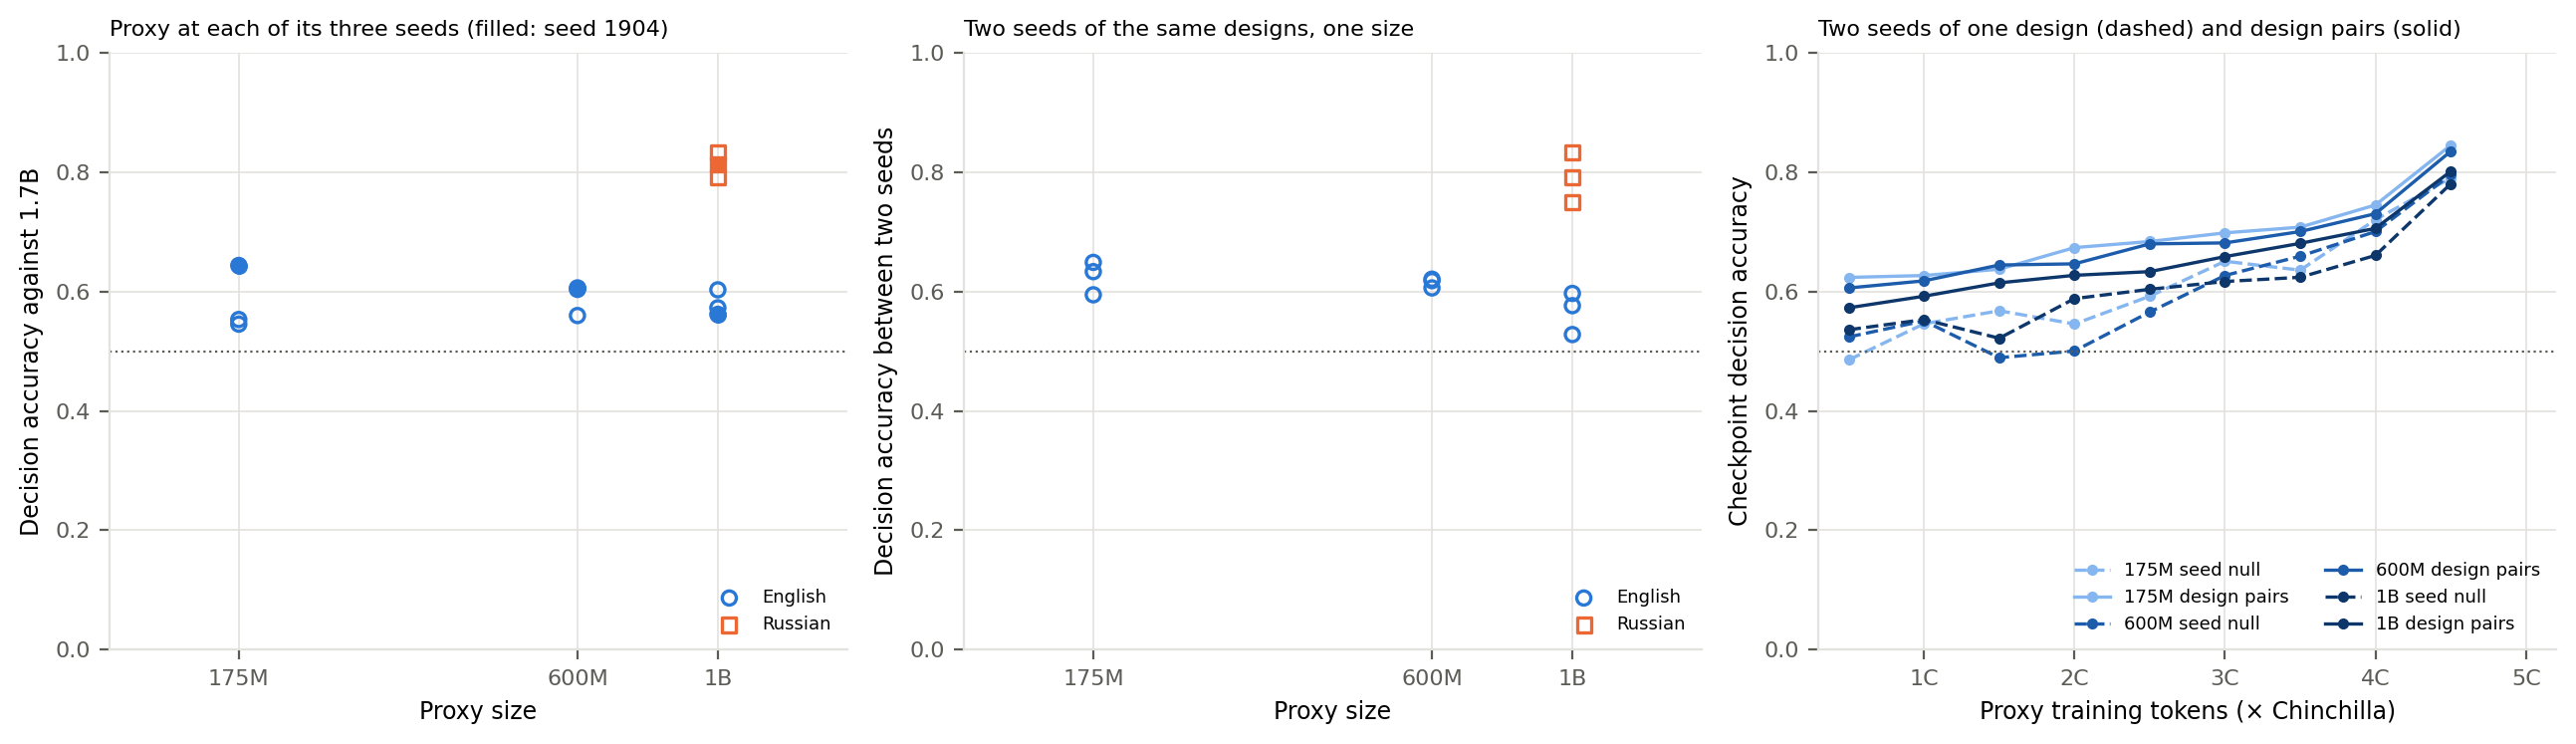
\includegraphics[width=\textwidth,height=0.8\textheight,keepaspectratio]{figures/app_rq02_seed_uncertainty.png}
% source: src/signal-and-noise/analysis/rq02_decision_accuracy/pretraining/predictivity/seed_uncertainty_da_all_seed_null_paper.png
\caption{\textbf{Two seeds of one design agree with each other about as often as a proxy agrees with the reference.} Left and middle: the replicated cells only, English at 175M, 600M and 1B and Russian at 1B, the deep cells with the baseline data trained with three seeds, pooled over tasks. Left: DA-size of the proxy at each of its three seeds against the 1.7B final checkpoint (filled: seed 1904). Middle: the agreement between two seeds' rankings of the same designs at one size. Right: DA-ckpt of the pairs formed by two seeds of one design, which have nothing to decide (seed null), against the real design pairs, over the evaluated checkpoints of each size. Every task above chance, bBPB twins included.}
\label{fig:app_rq02_seed_uncertainty}
\end{figure*}
